In addition to the CUDA framework on NVIDIA GPUs, the Open Computing 
Language (OpenCL) provides another standard for programming on GPUs.
%
OpenCL is supported by more venders, including Apple, AMD, NVIDIA, Intel, 
IBM, etc., because it is an open standard.
%
The main advantage of OpenCL is its portability across multiple devices and 
capability for heterogeneous computing.
%
In the following subsections, I will briefly introduce the programming 
model of OpenCL, 
then provide a use case of performing DWT on OpenCL, 
and finally compare OpenCL with CUDA.


\subsection{OpenCL Programming Model}
\label{sec:opencl-model}
%
Sharma et. al. provide an overview of the OpenCL programming 
model~\cite{sharma2010parallel}.
%
This programming model shares the same structure as the CUDA model.
%
In the finest level, each thread is named as a ``work-item".
%
In the coarser level, many work-items are put together as a 
work-group. 
%
The work-groups here are similar to the blocks in a CUDA model. 


In terms of the memory model, the global memory is shared between all
work-groups, while the local memory is shared by work-items in 
a particular work-group. 
%
Each work-item, then, has its private memory, which are essentially registers.
%
Figure~\ref{fig:opencl-model} illustrates this memory model.

\begin{figure}
    \centering
    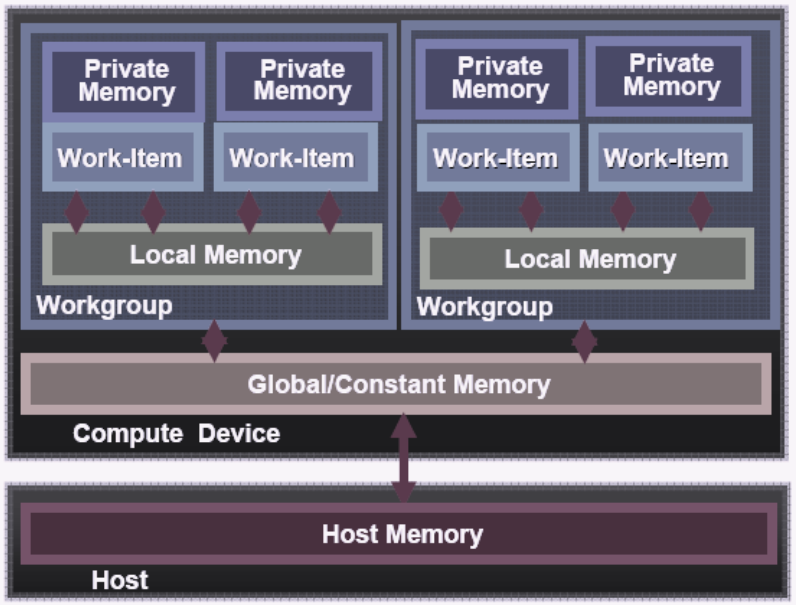
\includegraphics[width=0.8\textwidth]{fig/opencl-model.png}
    \caption{The OpenCL memory model}
    \label{fig:opencl-model}
\end{figure}


\subsection{Comparison Between OpenCL and CUDA}
\label{sec:opencl-cuda}
%
As an open standard, OpenCL is supported by both NVIDIA and ATI.
%
Sharma et. al.~\cite{sharma2010parallel} and 
Bernabe et. al.~\cite{bernabe2012cuda}
studied the performance comparison between OpenCL and CUDA


In the performance comparison study, the researchers implemented DWT
using the same algorithm, in both OpenCL and CUDA framework.
%
The test was run on an NVIDIA card, since that is the only GPU vender 
that supports both frameworks.
%
The performance of memory access and kernel calculation is evaluated separately.


The first set of experiments compare different memory access patterns.
%
The overall results suggest that OpenCL memory accesses are slower than CUDA,
with great variation from some API calls to others.
%
More specifically, the OpenCL performs as bad as 6x slower than CUDA using 
some API calls, while exhibits same results in some other API calls.


The second set of experiments compare the kernel codes that actually
perform the calculation.
%
Similar to the memory access tests, OpenCL implementations perform
poorer than CUDA implementations.
%
But interestingly, the slow down of OpenCL has much smaller variance
--- it is up to $72\%$ slower than CUDA.



While all the test results are strongly in favor of CUDA rather than 
OpenCL, I notice that all these tests are run on NVIDIA GPUs. 
%
Given the test results that some OpenCL APIs perform better (e.g. 
close to CUDA) than some others, it is quite possible that NVIDIA puts 
more effort optimizing those good-performing API calls.
%
More experiments and studies are needed to draw a more thorough 
conclusion on the comparison between CUDA and OpenCL.
 
